\begingroup
	\usetikzlibrary{calc}
	\pgfdeclarelayer{dibujo}
	\pgfsetlayers{dibujo, main}
	\tikzstyle{zero}=[circle,draw=black,fill=gray,inner sep=0pt,minimum size=2.5mm]
	\tikzstyle{one}=[circle,draw=black,fill=black,inner sep=0pt,minimum size=2.5mm]
	\tikzstyle{two}=[circle,draw=black,fill=white,inner sep=0pt,minimum size=2.5mm]
	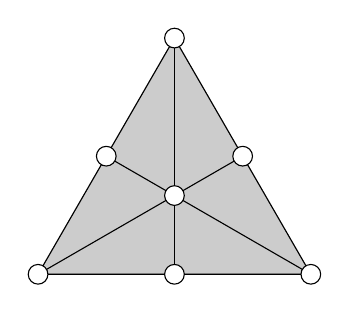
\begin{tikzpicture}
		\node [two] (bar) at (0,0) {};
		\node [two] (a) at (0,2) {};	
		\node [two] (b) at ($ (0,0) ! 1 ! 120:(0,2) $) {};
		\node [two] (c) at ($ (0,0) ! 1 ! 240:(0,2) $) {};
		\node [two] (x) at ($ (a) ! .5 ! 0:(b) $) {};
		\node [two] (y) at ($ (a) ! .5 ! 0:(c) $) {};
		\node [two] (z) at ($ (c) ! .5 ! 0:(b) $) {};
		\begin{pgfonlayer}{dibujo}
			\filldraw [fill=black,opacity=0.2] (0,2)--($ (0,0) ! 1 ! 120:(0,2) $)--($ (0,0) ! 1 ! 240:(0,2) $)--(0,2);
			\draw (0,2)--($ (0,0) ! 1 ! 120:(0,2) $)--($ (0,0) ! 1 ! 240:(0,2) $)--(0,2);
			\draw (0,0)--($ (a) ! .5 ! 0:(b) $);
			\draw (0,0)--($ (c) ! .5 ! 0:(b) $);
			\draw (0,0)--($ (a) ! .5 ! 0:(c) $);
			\draw (0,0)--(0,2);
			\draw (0,0)--($ (0,0) ! 1 ! 120:(0,2) $);
			\draw (0,0)--($ (0,0) ! 1 ! 240:(0,2) $);
		\end{pgfonlayer}
	
			
	\end{tikzpicture}
%	\label{fig:2_simplex}
\endgroup